\chapter{Discussion}\label{chap:discussion}



This chapter will discuss the obtained results, the used methodology, the validity and the reliability of the experiments, adapting the structure proposed by \textcite{luckert2016using}. Section \ref{sec:results-interpretation} will look into the results, describing what has been achieved, as well as indicate the main problems concerning the experiments. Section \ref{sec:method-reflection} will reflect on the research task and discuss whether the right method was chosen to solve the given task. Finally, Section \ref{sec:results-reliability} discusses the validity of the datasets that were used and the overall experiment setup. Based on these validity remarks, this chapter will clarify the reliability of the experiments' results. Therefore, the following questions will be tackled:
\begin{itemize}
    \item What conclusions can be taken from the presented results?
    \item Was the chosen method appropriate for the task?
    \item What benefits and shortcomings have been identified related to the presented work?
    \item What is the validity and reliability of the used data sets and the presented results?
\end{itemize}


\section{Results Interpretation}\label{sec:results-interpretation}

 The following sections present the results for the object-focused agents and environment-focused agents. Mixed-focus agents that explore both octrees and objects are discussed further below in Section \ref{chap5:mixed-focused}. The results are presented from each knowledge-based perspectives. 
%  These perspectives allocate the results according to the research question they answer to. 
 Voxel knowledge is provided when voxel elements are visible in the grid sensor view to the agent, Similarly, octree knowledge is provided through octree node observations, pigeon observations or observations of the lingering metric. This should allow the validation of our approach against other methods.
 
    \subsection{Object Exploration with Knowledge of Voxels} 
        %among all object-focused agents
        In general, the best performing object-focused agent without any semantic information has "oracle" knowledge about the nearest goal. 
        As expected, this shows that oracle observations (walk and look angles towards the closest goal) contribute towards finding objects faster, since these agents have more information about the environment.
        Surprisingly, the best agent is run \textit{voxel-entropy++100-nospeed}, which scanned an average of 2.10 objects per episode with a standard deviation of 0.2. This agent has vision of voxels and also observes the level of entropy in the scene around it through the observation \textit{LingeringPenaltyStrength} (see equation \ref{eu_lingeringpenaltystrength}).
        This agent is closely followed by oracle run \textit{voxel++100-nospeed-nolinger-oracle-8}, which scans an average of 1.77 objects per episode, and its non-oracle variant, \textit{voxzel+100-nospeed-nolinger}, which scanned 1.73 objects per episode. 
        % Close in performance was \textit{run63+100-nospeed}. 
        
        Overall, the training results show that the best object exploration results were achieved by the agents that had a \textit{sparse high voxel reward function}. In other words, the best performances were achieved when the agents can focus on the scanning of voxels without the distraction of other reward functions. 
        Accordingly, the mechanism to reduce the minimum speed penalty and the lingering penalty, if voxels were found in the agent's field of vision (FOV), did not provide the expected performance in \textit{run63++075}, nor \textit{run63++100}.
        However, even though \textit{run63++025} had the influence of the minimum speed penalty and the lingering penalty, its performance was almost as high as the aforementioned runs with 1.56 objects scanned per episode. This indicates the pressure to change the behavior in the presence of voxels was relieved through a smaller voxel reward (25\%).
        
        These results points towards the hypothesis that a high voxel reward function diverges from the reward signal of these penalties. 
        Therefore balancing these two priorites can be challenging for the agent if the voxel reward is set as a priority by the domain experts.
        It can also be inferred that simpler agents with clear goals and fewer distractions perform better at scanning the objects they need. 

        % Table \ref{tab:results-RQ1-explorative-performance} also shows that the minimum speed penalty had a negative impact on the explorative capabilities of these runs. Concretely, agents without a minimum speed penalty visited an average of 36-40 octree leaf nodes and perceived an average of 119-131 octree scan points, with an octant setup of 4$m^3$, whereas other agents visited an average of 29 leaf nodes and perceived 87-90 scan points. 
        
        % In contrast, \textit{run63++075} and \textit{rurn63++100} were able to scan an average of 0.96 and 0.77 total objects per episode respectively, with a standard deviation of 0.17, and visit 
      
        An additional point of interest is the fact that some agents prefer to move to a newer object before fully scanning the first one.
        % some agents lack the motivation to finish scanning objects. 
    % is to test the change in performance with an added
        % This would motivate the agent to scan all voxels of an object before moving to a new one. 
        In situations where the training setup allocates multiple objects close to each other, the agent chooses to initially scan the visible sides from each object instead of scanning the objects sequentially.
        Even though this behavior could be adjusted with a reward for finishing the full scan of an object, it is also explained by the pressure the agent has from the movement penalties. 
        An alternative solution would be to reward the agent for moving at a slower speeds when voxels are in the agent's FOV.
    %    behavior could also be adjusted by rewarding
       
    %  Animal... In general All methods with Oracle information Achieve high performance Oracle methods with an average of 1.7 Object scan per episode, from the best performing ones Bad band 
    %     From the runs that had no information about The position of the object in the 3D space   
    %     Concretely,
    
        % were under the pressure of a, perform better at exploration
        On a separate note, the shortest-path agents did not perform as expected and were greatly out-shined by the oracle agents. 
        The difference between these two agents is that oracle runs have shortest-path observations, but do not receive a penalty from the walk and look errors. 
        Visual inspection showed that the penalty for the walk and look errors caused the shortest-path agent to fly above goals to try to minimize these errors, instead of focusing on scanning the voxels. This also indicates that the walk and look penalties were too high in comparison to the rewards given for scanning voxels.
        Finally, the FOV-reduction mechanism did not improve these agent's performance within the 30M training timesteps, which suggests that the behavior adjustment should be looked at from a different perspective, such as action masking \cite{github-unity-mlagents-toolkit}. This would limit the agents behavior at a "hardware" level.
        
        
        \begin{figure}[!ht]
        \centering
        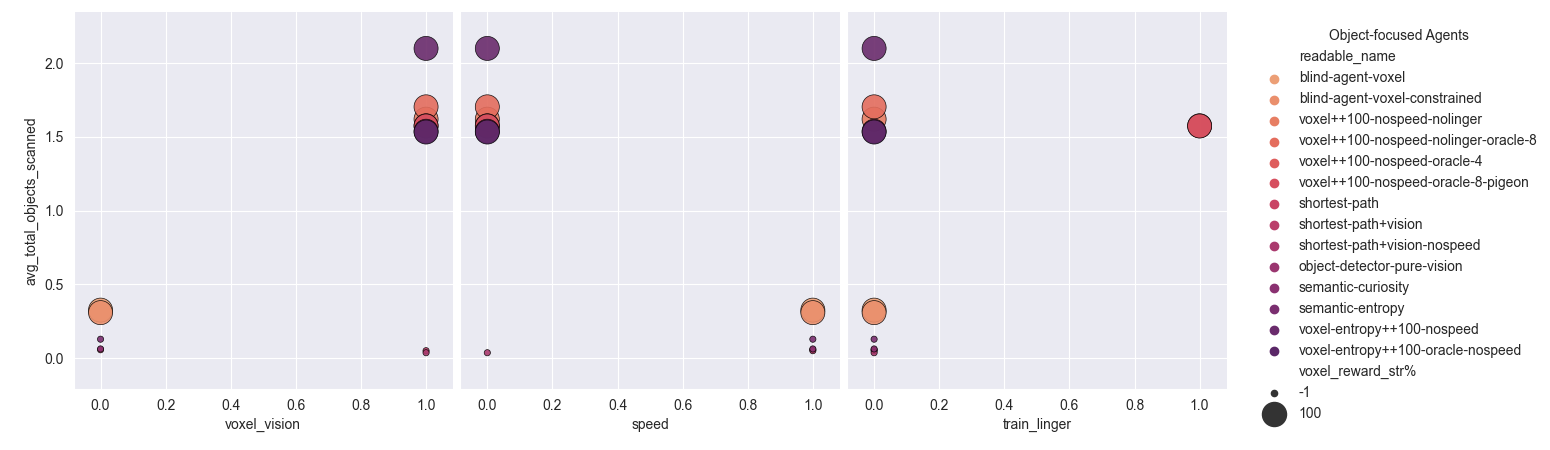
\includegraphics[width=1\textwidth]{images/results_variables_obj3.png} 
        \caption{Comparison of the influence of relevant variables on the total amount of objects scanned, for a subset of the voxel-focused runs. The variables for \textit{pigeon} and \textit{pathak} are always set to 1 (active).}
        \label{fig:results_variables_obj}
        \end{figure}
        
        It is also important to consider the question of what observations, rewards, and constraints have the greatest impact on the effectiveness of agents in solving particular tasks.
        Based on the performance of runs below the 25th percentile and above the 75th percentile, Figure \ref{fig:results_variables_obj} visualizes the influence of the most relevant variables. 
        Results show that voxel-aware agents without the minimum speed requirement perform better when the voxel reward is over 75\% strength, which corresponds to the performance discussed above.
        % Similarly, the agent with a weaker voxel reward could balance with these penalties, at 25\% 
        Finally, the constraint variable confirms that only agents without a normalized voxel reward signal saw sufficient value in the collection of voxels to overcome the penalties of environment. 
        For example, \textit{blind-agent-voxel} only explores a volume of 77 $m^3$, which, on visual inspection, is the space it covers spinning in circles, minimizing the minimum speed penalty. For more detailed plots on the variable influence for all runs please refer to Appendix \ref{appendix:agent_variables_influence}.
  
        % Given 6 objects in the scene, the best runs do not explore more than 5\% the environment. This metric is highly dependant on the fact that there are many objects in the scene. Moreover, this metric might also be skewed given collision problems displayed in the visual performance analysis of the drones. More concretely, the best performing agents were very fast at scanning objects, but sometimes they would "crash" against an object and stay still, "stuck" for the rest of an episode.
    
        % This behavior drags the overall average leaf nodes metric down.
        
        % One reason for this behavior could be the training time scale chosen. It has been reported that training at higher time scales can break physics interactions and collisions [ref unity forum]. However, we have chosen a time scale of 20 to avoid such problems.
        
        % However this has proven to be caused by the \textit{collision detection} method set for the \textit{rigid body} of the agent. The initial collision problems were caused by the discrete detection method. Rigidbodies with more active movemement like our drone should prefer to use a variant of the continous detection methods Unity provides. We have chosen to run inference with an speculative collision detection, since our use case does not require fine measurements when the drone collides against obstacles in the scene.
        
        % Something to also consider is the movement algorithm in the agents. It would be interesting to take a closer look at the movement algorithm and even allow the agent to move both left and right at the same time, instead of only left or right. This would provide more freedom in movement according to the situation. 
          
        %   to consider in to consider 
        % \textbf{Mixed-focused agents.} This contrasts, however, with the mixed-focus variants' performance.. 
        % \textit{runs63++025}, which demonstrate that he agent to forget about the minimum speed constraint and focus on scanning the voxels, achieving a similar behavior to \textit{run63++025}. In contrast, 
        % the manual manipulation of features "MAV", with a 0.67 cm error with a standard deviation of 2.46. 
        % The variations of MAV do not show substantial differences, yet they all present an average error higher than 0.5 mm with respect to the ground truth. 
        % The best results among all algorithms for the first research questions were achieved by
        % This contrasts with the other two algorithms, the 
        % An additional subject of interest is the comparison of res
        % Something to consider is that some agents do not finish sc
        % Furthermore, the questions of, which observations and which rewards have the most influence to solve the given problem
        % is an important topic to address. An analysis has been done on the results o
        % This example has been chosen, since it represents the most commonly used attributes for
        
        % Furthermore, as shown in table 4.10, using Google Translate as a candidate, results in
        % substantially higher recall values for automated translation and therefore higher precision
        % values for professional translation
        
        % Assuming, that all Google produced sentences share a characteristi
        
        % The addition of a round-trip translation to be used as 
        
        In summary, the best performing agent achieves an average of 2.1 total objects scanned while only visiting 147$m^3$ of the environment per episode. This agent is also characterized for performing better when removing the minimum speed penalty and, tentatively, the lingering penalty. 
        It is worth reminding that goals are situated at the ground level of the environment and not at different heights, which does not motivate the agent to explore remote locations of the environment to find the goals. 
        % Therefore, 0.79\% of the environment covers approximately an area of 124 square meters (octree nodes of size 4). 
    %  divided through octree nodes of 4 meters equals 31 leaf nodes approximately, or an area
    
    
        % Summarizing, the best achieved results show a classification accuracy of 72:24%, resulting
        % in a gain over a random classifier of 22:24% using Bing Translator as a candidate and
        % Google Translate as a pseudo reference.
    

    \subsection{Object Exploration without Knowledge of Voxels}
        This section discusses the results for the agents that receive a voxel reward but are not directly able to see voxels in their grid sensor view.
        
         While we expected the \textit{semantic-curiosity} agent to be the best run, the best \textit{blind} agent is \textit{object-detector-nospeed} with an average of 0.94 objects scanned per episode. The \textit{semantic-curiosity} agent however has the highest detections count per episode: visual inspection shows that the agent moves towards objects to scan them but is not as accurate as the \textit{object-detector-nospeed}. We suspect this occurs because the \textit{RationalizedClassEntropy} (see equation \ref{eu_rationalized_class_entropy}) uses temporal information across the past 10 frames, whereas the \textit{object-detector-nospeed} use of the immediate output of the object detector translates to more recent signals.
        
        
                % This variant proved its performance in the previous section with run \textit{object-detector-pure-vision}, which achieves an average of 1.54 objects scanned per episode.

        Overall, the results show that these agents struggle to scan voxels of objects without their explicit vision. 
        On the one hand, the shortest path agent was overwhelmed by the penalties from the walk and look errors, scanning an average of 0.06 objects per episode. 
        On the other hand, the semantic curiosity agent prefers states that maximize Chaplot's rationalized class entropy \cite{chaplot2020semantic}. 
        Such states are usually too far from voxels and prefer locations where multiple objects are in the agent's camera view (given the late update received from the temporal buffer). 
        Such performances were achieved similar scores as the random agent. Additionally, fully blind agents, which do not observe any information nor penalties, performed better with 0.39 objects scanned per episode. 
        % To distinguish if the performance of these methods was solely due to the lack of voxel-vision, voxel-aware variants were trained. Results show, however, that these methods lay the wrong focus on the object exploration task, with the exception of run \textit{object-detector-pure-vision}, which achieved an average of 1.54 objects scanned per episode.
       
        % In order to improve the performance of these methods, the penalties and reward strengths would have to be restructured. similar to what was done with the shortest-path algorithm, where voxel-agents were given only the observations under the suffix \textit{oracle}.
        
        Concluding, among agents that do not have knowledge of voxels, the object detector agent performed the best with 0.94 objects scanned per episode. In order to improve the performance of these methods, we suggest that the penalties and reward strengths would have to be restructured.
        % in comparison to other blind agents, knowledge about voxels and scarce reward functions proved to achieve better performance in the object exploration tasks.
        % 
            % Results show that mixed-focused agents achieve an even better performance 
                
            % Due to the lack of a sufficient amount of technical documents to train machine learning
            % algorithms on a document level, the approach to classify documents into the classes professional
            % translation and automated translation consisted of 
            
            % To increase the significance of the document-based approach, an additional 19190 manufactured
            % documents were ta
            
            % An important fact concerning the original document, are the clearly visible differences in
            % prediction distributions. 
            
            % Another important point of concern, is the question of the percentage share distribution
            % of the respective labels. T
            
            % It is clearly visible that longer documents deviate less in terms of classification distributions
            % than shorter docu
            
            % Based on the performance of the best runs Figure \ref{fig:results_variables_obj} visualizes the influence of the most relevant variables.
    
            % % Furthermore, as shown in table 4.10, using Google Translate as a candidate, results in
            % % substantially higher recall values for automated translation and therefore higher precision
            % % values for professional translation
            
            % % Assuming, that all Google produced sentences share a characteristi
            
            % % The addition of a round-trip translation to be used as 
    
    
            % Concluding, although the algorithm classifies every document with one of the two given
            % classes, the results cannot always be taken for certain, since the resulting percentage share
            % of sentence level classification plays an important role for determining the certainty of
            % the classification. The present approach proposes a classification with certainty, if the
            % classified document fits into one of the following areas:
            %  C1, D1 for a classification with professional translation or
            %  C2, D2 for a classification with automated translation.

    \subsection{Environment Exploration with Knowledge of Octrees}
        
        This section explores the results for the agents that are rewarded for exploring new locations in the explorable environment, with observations such as the amount octree nodes discovered or pigeon observations. 
        
        The best performing octree aware agent was \textit{octree-4}, which discovers 348$m^3$ of the environment in the maximum 5000 timesteps given. It is closely followed by \textit{octree-16-constrained-pigeon} which discovers 325$m^3$ of the environment. 
        % Regardless of the limitation that each training episode is limited to
        It is worth noting that each different octree node size provides a different amount of granularity about the positions in the environment: unlike a 16-meter-wide leaf node, a 4-meter-wide leaf node requires an agent to visit more precise locations in the environment.
        This is observed in the amount of nodes that constitute the explorable 3D volume at each different dimension (4000, 500 and 62.5). 
        In essence, exploratory capabilities do not vary with the size of the octree node. However, bigger octree node sizes promote the agent to visit more dispersed locations of the environment.
        Whereas the performance of \textit{octree-4} accounts for 2.18\% of the 4000 leaf nodes in the environment,  \textit{octree-16-constrained-pigeon} covers almost 33\% of the 62.5 leaf nodes in the 5000 timesteps given. 
        % The best exploratory capabilities are demonstrated by octree explorers that use node sizes of 16 meters: they prove that agents can visit several spaced-out locations in the limited time given.
        % Factors like the 
        
        % As mentioned in section 3.3 there was reasonable concern that the amount of existing at-
        % tributes using no reference translations was insufficient to create a useful classifier for the
        % given problem. 

        % The agent with 16 nodes is capable of "covering" much more space 
               
        % Based on the performance of the best runs Figure \ref{fig:results_variables_octree} visualizes the influence of the most relevant variables.
        
        Another positive point of interest is that the pigeon observations provided a positive impact on exploration missions and helped agents better orient themselves in a mapless environment and cover more different locations, as shown by run \textit{octree-16-constrained-pigeon}'s 33\% coverage 
        Interestingly, Pathak's curiosity module did not provide added value to run \textit{octree-16-constrained-pigeon-pathak}, bringing its coverage percentage to 9.5\%.
        
        Furthermore, the constraint variable proved itself useful to evaluate the performance agents that end the episode too soon. This occurred when the rewards were too low or the penalties too high, such as in the case of runs  \textit{octree-16} and \textit{octree-4-pigeon}. 
        % It is cleIt is unclear why octree agents chose to exit the environment. One hyptthesiss
        % that runs with a smaller leaf note size have the highest episode length among the unconstrained runs
        % I expected the constrained runs collect the highest episode length

        % Furthermore, as shown in table 4.10, using Google Translate as a candidate, results in
        % substantially higher recall values for automated translation and therefore higher precision
        % values for professional translation
        
        % Assuming, that all Google produced sentences share a characteristi
        
        % The addition of a round-trip translation to be used as 

        These results suggest that octrees are appropriate navigation data structures to reward the agent for navigating new locations in an environment. It is important to highlight that the agent does not have access to the octree nodes nor some kind of map. 
        Our best octree-only agent is able to explore 348$m^3$ of the environment in 132 seconds using uniquely the reward per each new octree node visited. We are certain that this coverage would be higher given a higher episode limit, as shown in the to-be-discussed test results.
        % However, our mapless agent that, similar to pigeons, uses a magnetic north and the position of the sun to determine a relative overall position in the map, achieves 34\% coverage of the space in the given 5000 timesteps. 
        
        % This represents a distance of about 340 meters, crossed , without repeating.
        % This corresponds to approximately 340 meters traversed 132 seconds without repetition. 
        % \ref{https://johnaustin.io/articles/2019/fix-your-unity-timestep#:~:text=Each%20Update%20pass%20actually%20spans,the%20game%2Dtime%20between%20frames.}.
    
    \subsection{Environment Exploration without Knowledge of Octrees} \label{chap:5:discussion-env-exploration-wout-octrees}
  
        This section discusses the results for agents that are rewarded for visiting new octree nodes, yet do not have any information about the number of octree nodes discovered nor spatial information such as pigeon observations. This covers blind agents and those based on Pathak's method \cite{pathak2017curiosity}. The latter is a 1-1 implementation of the paper and is provided through Unity ML-Agents' curiosity module \cite{github-unity-mlagents-toolkit}.
        
        Surprisingly, the best performing agent is \textit{blind-octree-explorer-nospeed}, which explores 364$m^3$ of the environment within 5000 timesteps. This suggests that the observations that \textit{octree-4} perceives (the number of octree nodes discovered) does not provide substantial change in the awareness of the octree. 
        Furthermore, these agents provide an explanation to the early-exiting of the environment by the octree agents: the minimum speed penalty overshadows the rewards provided by the discovered octree nodes. 
        
        % impthe exploratory performance of , an
         
        % This is because they cannot remember the locations they already visited. 
        % It is interesting to note that the relative location in 3D space does not provide the agent sufficient information for it to create an internal geographical consciousness model.
        % % Interestingly, the relative position of the agent in the 3D space is not enough information for these agents to create some sort of awareness model.  
        
        % Furthermore, due to differences in environmental coverage, these results must be interpreted with caution: an agent that covers 2\% of the environment with 4-meter-wide leaf nodes, could potentially cover 4 times as much if motivated by 16-meters-wide leaf nodes.
        % However, even with the adjusted results, these agents would cover only 20\% of the space of the best performing agent from the previous section.
        
        % Interestingly, \textit{pathak-16-constr-nospeed-nolinger}
        The best performing Pathak baseline is \textit{pathak-4}, which achieves 318$m^3$, which suggests that pathak does not contribute to the discovery of new octree nodes. 
        Interestingly, the removal of the lingering penalty in \textit{pathak-16-constrained-nospeed-nolinger} (304$m^3$ explored) shows an increase in performance compared to \textit{pathak-16-constrained-nospeed} (16$m^3$ explored), which suggests that the lingering penalty is not compatible with Pathak's reward function.
        
        % On a positive note, one of Pathak-derivated agents, \textit{pathak-4}, achieves a 7\% coverage and a potential 14\% coverage with a 16-meter-wide node. Agent \textit{pathak-16-constrained} demonstrates this by achieving \% coverage. 
        
        % Accordingly, \textit{pathak-16-constrained-nospeed} achieves \% coverage and shows that the speed parameter does not contribute to exploring more octree nodes. 
        
        % However, run \textit{pathak-16-constrained-nospeed-nolinger} explores \% of the environment and demonstrates that the linger penalty does benefit the exploratory capabilities of an octree-agent.
        
        
            % The results discussed above, were used to create a document-based classification system
            % similar to the one discussed in subsection 5.1.2. The results for the original documents are
            % shown in table 4.15. The first apparent fact is that in this case,
            
            % The evaluation shows an average misclassification rate of 32:81% for the shortest documents,
            % 25:98% for documents containing ten sentences and an average error of 4% for
            % document length 250 before dropping to 0% for larger test files.
            % As for Research Question 1, the senten
            
            
            % The areas of interest are the same as described in subsection 5.1.2. The deviations in the
            % areas of larger documents are due to the comparably small amount of created documents
            % for lengths of 1000 s
    
     
     
        These results broaden our understanding of the feasibility of octrees for the exploration of environments and the influence of the minimum speed penalty, the lingering penalty and Pathak's curiosity method. Overall, the results for the fully blind agents suggest that octrees are an appropriate data structure for motivating a agent to explore the environment. 
        It is safe to say that an explorer agent does not necessarily need a minimum speed constraint and that the lingering penalty's value function conflicts with Pathak's method when applied to exploration.
        
    \subsection{Mixed-focused Exploration} \label{chap5:mixed-focused}
        This section deals with the results from the mixed-focused agents. These agents balance the exploration of both objects and the environment. The baseline mixed-agent incorporates the voxel-entropy agent, removes the minimum speed requirement, and adds octree-node observations, pigeon observations and Pathak's curiosity module. 
        This set of results incorporate an F1-score metric, calculated from the total objects scanned and the octree leaf nodes visited metrics. 
        This allows the use of a single metric to evaluate the effectiveness of agents in balancing motivation between two high-level tasks.
        % This should allow the usage of one single metric to evaluate the harmony score of the agents that try to balance between two tasks.
       
        According to our F1-score, the best mixed-focus agent is the \textit{explorer-entropy-8}, with a 0.3 score. This result, however, comes at the expense of exploring less of the environment (151$m^3$) and scanning more objects (1.96). The best mixed-agent for exploration is agent \textit{explorer-entropy-4-noTrainEntropy}, which covers 358$m^3$ of the environment. This result shows that the agent prioritizes the exploration of the environment over the scanning of voxels. This is because the octree reward is higher and is present at every timestep, whereas the voxel reward is sparse.
        % in comparison to the voxel reward, 
        % scanning fewer objects (1.20) and exploring more of the environment (8\%). 
        % Nevertheless, our preferred best agent is the runner up, \textit{explorer-entropy-8}, since it scans almost twice as many objects per episode and achieves a similar corrected leaf nodes coverage. This claim might seem counter-intuitive, since the results show that an agent with fewer octree-rewards should focus on object scanning. However, the reader must remember that, as previously mentioned, the percentage of coverage for \textit{explorer-entropy-8} must be multiplied by a factor of two to be compared to any variant of \textit{explorer-entropy-16}. 
        % This results in the corrected octree leaf node coverage percentage. 
        % Along these lines, it is also safe to claim that \textit{explorer-entropy-16} does not perform as well as \textit{explorer-entropy-8} since, given such a small reward in the environment, the agent is negatively distracted by the lingering penalty being modified by the semantic entropy modifier. 
        
        Another point of interest is that the results show that agents the adjustment of the \textit{LingeringPenaltyStrength} (see equation \ref{eu_lingeringpenaltystrength}) did contribute to both the exploration of the environment and of objects. Concretely, \textit{explorer-entropy-8-noTrainEntropy} is the runner-up agent with an average of 1.65 objects per episode and explores 139$m^3$ of the environment. 
        Furthermore, the lingering penalty positively influenced the performance mixed-focus agent: \textit{explorer-entropy-8-nolinger} explored less of the environment (117$m^3$) and less objects per episode(1.77).
    
        % agents, as shown by \textit{explorer-entropy-8-nolinger} Instead, agents that did not modify the lingering penalty strength, such as \textit{explorer-entropy-8-noTrainEntropy} performed better than agents that removed it altogether, for instance, \textit{explorer-entropy-8-nolinger}.
        
        % As a reminder, the semantic entropy modifier regulates the strength of the lingering penalty based on the rationalized entropy observed by the object detector. This claim is supported by the performance shown by \textit{explorer-entropy-16-nolinger}, which achieves similar octree-explorative performance as the best run. Finally, the difference in objects scanned is justified by the unnecessary observation this agent receives: the value of the lingering penalty strength is changing yet it is not directly related to any reward or penalty, given the \textit{-nolinger} suffix.
        
        
        % The reader must remember, as mentioned before, the corrected octree leaf nodes coverage percentage for the 8-meters-wide leaf nodes must be multiplied by a factor of two to be compared with the explorers that use 8-meters-wide leaf nodes.
    
        % Additionally, it is safe to say that Pathak's curiosity ML-Agents module contributes to finding new states, yet an analysis on the impact of fine tuning its hyperparameters would be important.
        Taken together, these findings demonstrate that mixed-focus agents are capable of balancing the object- and environment-exploration tasks.
        % agents with simpler, consistent reward signals, without unnecessary penalties, provide the best performance. 
        In addition, it can safely be said that Pathak's curiosity module provided by ML-Agents helps agents find new states, but it would be important to analyze the effects of fine-tuning its hyperparameters.
        % confuse the agent about which signal is the correct  are actually related to the penalties or rewards being given. 
        % Furthermore, these noise observations
        % and observations should be avoided at all costs
        Finally, even though counter-intuitive, the removal of the minimum speed requirement suggests that noise (unnecessary) rewards (and observations) should be avoided, as they translate into slower convergence times and they mask which observations actually matter for the task at hand.
        We hope that these findings will reach RL practitioners, specially those who were also inspired by \citetitle{silver2021reward}\cite{silver2021reward}, so that observations and rewards will be carefully deconstructed, analyzed, and evaluated for their actual impact on an agent's behavior.


    \subsection{Comparison of the two Research Questions}
    % TODO HERE:
        Regarding the setup of the two research questions, each research question (RQ) tackled a different expected policy in the reinforcement learning agent. While RQ1 focuses on the exploration of objects from multiple angles, RQ2 deals with the exploration of unknown environments, in which objects of interest could be found. The usage of Unity 3D provided a platform for the implementation and practical testing, in addition to the theoretical argumentation of our approach.
        Furthermore, the separation of methods based on knowledge about octrees or voxels, allowed the critical, unbiased, feasibility evaluation of our proposed approach.
        The expected results were that agents trained with knowledge of voxels and octrees would balance both policies and even outperform single-task agents and the chosen blind-baselines, following Silver's claim \textcite{silver2021reward}. These expectations were confirmed by the experiments, achieving over 2 scanned objects per episode while covering a minimum volume of 147$m^3$ without repetition. 
        
        From the perspective of RQ1, the our best mixed-focus agent shows an increase in the amount of objects scanned by at least a factor of two in comparison to the best chosen baseline (object detector). Moreover, this agent also shows an increase of 24\% compared to the best voxel-oracle run, \textit{voxel++100-nospeed-nolinger-oracle-8}.
        In comparison to our best voxel-focused run, \textit{voxel-entropy++100-nospeed}, our best mixed-focus agent is 7\% behind with 1.96 objects scanned.
        The respective results for the different algorithms are influenced the most by the minimum speed penalty, which added pressure on the agents to continue moving even though they needed to slow down to scan objects.

        From the point of view of research question 2, the best octree-focused agent \textit{octree-4} explores 5\% than the best baseline agent \textit{blind-octree-explorer-nospeed}. This points out that the amount of nodes discovered per timestep does not provide much "awareness" of the surrounding octree to the agent. This is one of the assumptions taken in this thesis work as part of the scope limitation that form part of the further steps. In other words, providing the octree agent with more information about the surrounding octree nodes (partial observability) would have expanded the scope of this work to analyze more aspects such as efficiency and performance variations given the three different types of octree nodes our data structure stores (scan points, visited points, out-of-range points). This allows for the continuation of this work to analyze the various possibilities that octrees can enable.  
        % On a separate note, the pigeon observations proved to be a valid mapless alternative to provide environment-agents with global orientation without direct map knowledge.  
        
        %To this, the blind-agents proved that the observation of the number of octree nodes per step does not provide meaningful information to the agent.
        % In contrast

        Accordingly, our best mixed-focus agent explores 59\% less the best environment-focused agent \textit{blind-octree-explorer-nospeed}. 
        % Concretely, the best environment-focused agent performs 53.5\% better than the best mixed-focus agent. 
        Similarly, Pathak's baseline \textit{pathak-4} falls 8\% behind our best environment-focused agent and 111\% ahead of the best mixed-focus agent, 
        This is expected due to the fact that mixed-focus agents must sacrifice their limited timesteps given, in order to explore the environment's objects.
        
        The respective results for the different agents that explore the environment are most influenced by the minimum speed penalty and the environment-reset-constraint variable. The removal of the former allowed agents to explore locations that required a slower speed, such as corners or around obstacles. Furthermore, though many of the early-stopping situations were caused by the minimum speed penalty, the addition of the environment-reset-constraint refused the agent the possibility of early-stopping episodes as a solution to the minimization of penalties, such as observed on 16-meter-wide subdivisions of the octree.
        
        
        % The figure above shows that the performance of blind methods is strictly lower than methods that had knowledge of voxels or octrees.

        
        It is important to remember that in the case of RQ1, we can only provide an approximate comparison in performance with relation to other state-of-the-art methods. The original methods were not implemented in the Unity game engine, and given the limited time scope, our implementations are not 1-1 copies of the original works. If the authors would be willing to adjust their solution to be tested in the Unity game engine, we can provide a much more accurate performance comparison. In the case of research question 2, our performance comparisons are reliable, since Pathak's curiosity module was implemented by the Unity ML-Agents development team as an identical copy of the method proposed by the original paper.
        
        Concluding, the experiments confirmed the expectations of octrees and voxels being able to balance the exploration of environments and objects. The in-depth analysis of the influence of observations and rewards in a reinforcement learning agent allowed the construction of an efficient, embodied explorer drone.
        
        % Concerning the setup of the two research questions, research question 1 was a more
        % straight forward task. Allowing the use of reference translations made the creation of
        % a valid attribute base easier and the results were more promising in the first optimization
        % runs. In contrast to that, the second research question created the problem of having to
        % solve a document quality problem without access to semantics of the document, since the
        % use of reference translations was not allowed. The addition o
        
        
        % Furthermore, the misclassification rate is clearly higher 
        
        
        % The figure above shows that misclassifications are strictly lower for every d
        
        
        % To further examine the performance between the two systems, it is important to look at
        % the percentage share of the different distributions rel
        
        % Based on the performance of the best runs Figure \ref{} visualizes the influence of the most relevant variables.
        % It is interesting to see that intrinsic curiosity from Pathak's method \cite{pathak2017curiosity} did not provide much value in the expiration task.
        
        
        % Concluding, the results of the experiments confirmed the expectations with research question
        % 1 being easier to solve using classification techniques, than research question 2, due
        % to higher overall and averaged accuracies on a sentence level, smaller misclassification
        % rates and more certain classifications for all sizes of documents.


    \subsection{Evaluation Framework}

        The proposed framework evaluates the performance of the agents based on two separate tasks, each corresponding to one research question. To this end, inspired by the DARPA Subterranean Challenge, two test environments were developed. One environment tests the agent's time-to-goal for three goals situated sequentially after the previous goal has been discovered. The second environment evaluates how much time each environment-curious agent takes to discover a proportion of the environment, up to 100\% coverage. Given the limited time scope, only the best training runs from four categories were tested: object-focused, environment-focused, baselines, and mixed-focus. For the tests, the length of each episode was extended from 5'000 to 40'000 timesteps. It is also worth mentioning that the episode length was not able to be set to infinite, since that simulations that run for too long without stopping required more computer memory than what we had available. Therefore, the percentages reported are for half of the explorable vertical space. 
        
        The results for the object-discovery task show that not all agents were able to reach the third goal within the given timesteps. Agents \textit{explorer-entropy-8}, \textit{voxel-entropy++100-nospeed} and \textit{voxel++100-nospeed} reached the third goal after 277, 357 and 264 seconds, respectively. They each have an average time between goals of 88, 92 and 119 seconds, and take an average of 1, 2 and 2 seconds/meter, respectively.
        These results show that the introduction of entropy as an awareness signal shows an impact in between the second and third best agents. They also show that our mixed-focus agent explores the environment faster and has overall better performance. 
        % Figure \ref{} shows the results for the object exploration task. 
        
        % Table \ref{} shows that 
        
        Concerning the environment exploration task, the results clearly show that not all agents are capable of exploring newer locations in the environment. 
        Firstly, given that baselines displayed a poor performance in the previous sections, it was expected that the baselines would not perform well in the test environments.
        Secondly, from the perspective of voxel-focused agents, it was expected that they are not able to explore much of an environment without goals. On visual inspection, the agents were stuck spinning around obstacles. 
        Thirdly, in terms of the mixed-focus agents, it was expected that they are able to perform to some extent in this test. Results show that they are capable of exploring the environment, but they are 11\% slower than the best agent for this task.
        % Since these agents are also trained for object-discovery, 
        Finally, results clearly show that a variant of the environment-focused agents was able to outperform all other agents. Concretely, run \textit{octree-16-constrained-pigeon-nospeed}, which uses 16-meter wide leaf nodes, was able to fully traverse half of the the environment (31 octree nodes) within 7.68 minutes. Its runner up, mixed-focus agent \textit{explorer-entropy-16-constrained} achieves the same result after 8.5 minutes.
    
        It can be therefore safely assumed that given an infinite episode (or an episode with at least 80 thousand timesteps), these agents would explore all of the environment after an average 16 minutes, covering therefore a volume of 62.5 octree nodes or a 100$m^3$.
        % covering .
        
        % There are multiple reasons for the 
        
        % Additionally, a weighted mistake count is added as additional context information. These
        % three attributes (a boolean value for the c
        
        % The mistake count had more influence on the sentence quality than the classification system,
        % resulting in most sentences with a mista
        
        % Concerning figure 5.6, it is clearly observable that Category 1 and 3 are the most frequent
        % classes, which is due to them c
        
        % It is clearly visible that the professionally translated documents are rated higher than the
        % respective automated documents. The reason for the professional documents being rated
        % with an average score of 2:00 is 
        
        % general interpretation

        % Our method performs surprisingly well in a,b,c
        
        % the model is robust to hyperparamter tuning, it is shown in the following comparisons under different setups 
        % the hyperparemeters tuned were

    
    % \subsection{Small Environment Performance}
    %     From the results of Section \ref{chap-4:small-env-results}, we observe two conclusions:
    %     \begin{itemize}
    %         \item Voxel-curiosity conclusion: The runs that perform the best are run 63 and 68, which are capable of seeing voxels and have no other distractions in terms of training. Interestingly,  Run65 (object detector agent) has shown significant improvements when the minimum speed constraint was removed. We conclude that having sparse and focused reward functions (voxels scanned) tend to a better learning (performing agent) in contrast to denser reward functions. Also in terms of rewards we see that the higher the voxel reward the more attention the agent gives to the collection of voxels, which is expected.


        
    %       \item Octree-exploration conclusion: The results in this run are quite clear: run62 (octree-only agent) is on the lead, since he does not have to split his attention to other tasks other than the discovery of the area. Accordingly, given the small area of 16 $m^2$, it is no surprise that most other runs perform similarly with an average reward of 0.04, since there is not much to be explored in this scene and the goal is only a few steps away from the agent's starting point.
    %     \end{itemize}
        
        
        % \subsection{PPO vs SAC}
        % We find that PPO can significantly improve sample efficiency while not being sensitive to hyperparameter tuning and also has a smaller variance than SAC. We show a few sample runs and present numerical results on a robot control task and a grid world navigation task. \ref{chap:4:summary} \ref{chap:5:robots}
    
    
    % \subsection{Panoramic Performance}
    
  

\section{Method Reflection}\label{sec:method-reflection}
    
    The used method to structure this thesis, adapted from the work by \cite{luckert2016using}, proved to be appropriate for proposing a solution for the research questions given. The format provided allowed for the setup of different experiments without neglecting the initial goal. From the identification of the goals for each task, through the environment description and the specification and proposition of the reinforcement learning approaches, the method proved to efficiently structure the work required to construct an octree- & voxel-curious explorer agent.

    Similarly, in terms of octree-focused agents, future steps would include the analysis of the performance of an \textit{octree-no-speed-pigeon} agent, given that results suggest that the addition of pigeon observations and the removal of the minimum speed requirement improved the exploratory performance of agents.

    Overall, the results of this work prove that octrees and voxels are suitable for finding a solution to the two research questions. To address analysis of possible reward signals capable of solving these tasks, multiple observations and reward signals were developed. These were then evaluated separately to determine their influence in the agent's behavior. Furthermore, combining the environment-focused agents with the object-focused agents allowed the final mixed-focused agents to balance both exploratory behaviors and reach outstanding performance in the evaluation framework. Finally, the abstraction of the complexities in the environment and of objects allowed the agent to be visual-agnostic and transfer the learned behaviors across the proposed practical scenarios from Section \ref{chap:4:practical-scenarios}. This demonstrates that our proposed method is capable of adapting to newer environments. 
    
    Furthermore, our method can be used as more than just an agent for navigation and exploration, but also as a baseline in the generation and evaluation of 3D object-centric datasets such as Objectron \cite{objectron2021dataset}, where the trajectories around objects to collect multiple perspectives about its features are essential for a thorough representation. Accordingly, in terms of the practical scenarios that are part of our contributions, it was important for us to cover three aspects in the creation of benchmarks, in order to continue the work laid out by Juliani et al. \cite{juliani2018unity}: 
    \begin{itemize}
        \item the contribution of data, which in our case comprise our Unity 3D environment setups.
        \item the provision of a baseline, which constitutes the diverse agents that are shipped with our deliverables.
        \item a new set of questions that will motivate further research in navigation, point-to-goal, dataset generation, online model training, reinforcement learning and active vision tasks.
    \end{itemize}

    Along these lines, it was most important for this thesis that the research carried out would distance itself with the common lack of reproducibility and dependency problems that clogs scientific research projects.

    To this end, not only does the usage of Unity 3D enabled the immediate reproduction of the experiments, but the ML-Agents plugin also proved to be a great toolbox for developing reinforcement learning agents. Concretely, it greatly simplified the development process with an intuitive UI, thorough documentation, an active and supportive community, and an extensive set of tools and modules such as attention, memory, curiosity, imitation learning, curriculum, and more.
    Ultimately, we consider ML-Agents an essential solution for developing reinforcement-learning-based solutions. The plugin, in cohesion with Unity, provided efficient means to model, evaluate and improve models and debug errors during the execution of the scientific method. 
    % The only current drawback from the Unity engine is the accumulation of memory if post-processing steps are not turned off manually. It is a debated topic, but it would be beneficial if the developers at Unity ML-Agents improved the handling of all post-processing effects that negatively impact training setups.
     
    Additionally, as part of the further use of the results, the evaluation of compatibility with as OpenAI Gym could be easily done with the OpenAI Gym wrapper provided with ML-Agents. The wrapper enabled the loading of our Unity-developed environments into a Jupyter notebook and Python scripts, where an agent could be trained using an external neural network from OpenAI Baselines \cite{github-dlr-rm-baselines3}.
    While the Unity OpenAI wrapper permitted a smooth environment transfer, the results presented in Section \ref{chap:4:cross-platform-compatibility} did not justify the overall usage of OpenAI Gym. 
    More concretely, development functions such as resuming of experiments, logging with Weights and Biases \cite{wandb2022}, debugging, etc., negatively affected the overall development process, which puts ML-Agents ahead of the curve. 
    % cross-platform development. 
    % he lack of out-of-the-box development 
    Even though Unity ML-Agents is currently limited to a set of trainers like PPO and SAC, it provided increased versatility and plug-and-play integration of a multitude of modules, such as attention, memory, curiosity, behavioral cloning, auto-curriculum, and many more. Therefore, we consider the use of Unity ML agents to be more appropriate for reinforcement learning tasks as of current writing. 
    % The only limitation of the plugin is that it is not possible to load externally created 3D environments.


    % The used KDD process proved to be suitable for finding a solution to the two research
    % questions. The standardized procedure allowed for the fle
    % To address possible translation system specific characteristics, three different machine
    % translation system
  
    
    % Focusing on the initial document quality evaluation on a sentence level ensured the significance
    % of the approach, since the used data set consisted of over 20:000 different sentences
    % in contrast to the original 14 doc
    % Besides the increased significance, 
    % However, the taken approach has a clear shortcoming. 
    
    Similarly, in small-scale environments, the results show that the longer an agent has to move to reach a goal, the greater the real difference in each method's effectiveness.
    % show that the longer the agent has to move to achieve a goal, the greater the actual difference in the effectiveness of each method.
    % there is an important difference in the actual performance of each method the longer the agent has to move to reach a goal.
    Concretely, large-scale environments prove that some agent behaviors are not motivated to explore to find rewards. Instead, these agents choose to move in circles in a small part of the environment, minimizing the minimum speed penalty. This indicates that these agents depend on the domain randomization to spawn a goal near them.
    In contrast, in small-scale environments octree agents are more predisposed to display similar performance, with at least an average of 23\% of the environment explored by all agents.
    % Others chose to move in circles, minimizing the minimum speed penalty, and to wait for the episode to restart. 
    % It is important to understand that even though 
    This proves that these methods are very effective in scanning voxels of objects in the vicinity, such as \textit{run65-pure} demonstrates after visual inspection. However, this does not translate to a policy that can be used in a practical environment.
    We can safely claim that "small environments" conceal the subtleties that could distinguish one method from another, since their performance metrics would not be too far apart. 
    Therefore, in order to properly assess exploration policies, we recommend that agents must face not only various scenarios with obstacles, different heights, shapes, and colors but also larger environments that resemble the real world.
    % We hope this helps the reader understand the fallacy of training exploration models in small environments. 

% This was observed by the performance of the \textit{ev\_smallcam.explorer-8}. 
    On top of that, the panoramic vision agents proved to outperform agents equipped with an ordinary monocular vision of 55 degrees. Concretely, while the \textit{smallcam} agent explored 278$m^3$ of the environment without scanning objects, its \textit{panoramic} alternative scanned 1.96 objects and explored 151$m^3$ of the environment per episode. These results support the claim by Zhang and Huang \cite{zhang2021panoramic} and research by Davison et al. \cite{davison2007monoslam}, presented in Section \ref{chap:3:gridsensors}, that monocular cameras require more complex models for target tracking, feature remembrance, additional noise reduction, etc. It is therefore safe to say, that panoramic cameras should be preferred in navigation tasks to avoid the unnecessary overhead small FOVs add in scientific research.
    % exploring 14.75\% of the environment. 
    
    
    % \subsection{Applicable Practical Scenarios} % Future
    
    % It should be noted that in training, many rendering effects, such as grass and moving clouds, do not always execute garbage collection mechanisms in the underlying system. This may result in a stop in training if the environment stops reacting due to a lack of remaining memory.
    % This may be a problem within Unity ML Agent's plugin episode reset logic, since this problem is not oberved in the test or demonstration runs.
    % Training was therefore carried out with the island presented in Chapter \ref{chap:4}, without any post-processing or special rendering effects.
    % This corresponded to an average memory usage of 9GB and a load of 60\% across 8 CPU cores, with 5 parallel training environments and a timescale of 20.
    % % Nevertheless, the trained agents were tested and fully functional in the applicable practical scenarios which demonstrated the possibility of transfer learning across environments and preserved the agent's explorative behavior.
    % As mentioned before, voxel-curious agents, which were trained on voxelized bikes, showed visual-agnostic behavior in other voxelized objects such as buses and homes.
    % This validates the proof of concept that our agents can be helpful in emergency rescue situations for police and firefighter drones, environment analysis in factories, airports, warehouses, in industries for defect analysis and product quality assurance, and more.
    



    % It is therefore up to the researcher o
    % in some area trying to minimize the minimum some of them trying to minimize the minimum speed requirement
        % Similarly when the object is only a few steps ahead the agent is not able the performance between agents the subtleties of the policies of each agent behavior cannot be distinguished because they all perform similarly

% \subsection{Cross-Scenario Performance}
    % Therefore approach expanded the target group of this master's thesis, where further applicability is possible, such as: police investigations, inspection of fire scenes by firefighter drones, factories, warehouses, airport robots, hospital robots, damage detection and analysis, etc. 
        
    
    % % \subsection{Cross-Platform Compatibility}
    % OpenAI gym showed similar performance to mlagents, but the toolbox that comes with it for 
    % took 80\% of the time invested, since    
    
      
    In terms of future steps, the following points were collected during the creation of this work, as great opportunities to continue research in reinforcement learning:
    \begin{itemize}
\item real-time voxelization of the objects of interest to capture limitations in terms of computing, memory and noise, while also considering efforts with event-driven cameras, inspired various works by Scaramuzza, such as \cite{messikommer2022bridging, muglikar2021event} and Grinvald \cite{grinvald2021tsdf}.


% noise in visuals when using a real translation from depth
\item a parallel-agent environment where multiple agents could be trained simultaneously. This is a relatively straight forward task using ML-Agents but given the limited time frame it could not be implemented given our setup. A separate but related point is a multi-agent learning and coordination, inspired by works by Jacques, such as \cite{ndousse2021emergent}.


    % but needs some engineering to load multiple configurations at the same time.
% \item a deeper argumentation on LiDAR's limitations at bigger distances and the benefit of cameras for navigation.
  
  
    % - clarification on: is this LiDAR behavior? >> leads to noise topic, because its not 100\% worth it now
    % - noise in scanner, how does the performance suffer ?
    % - simplified words: simplified SLAM and model free navigation.
    
    % Using different machine learning algorithms to evaluate the quality of sentences and even
    % documents, proves to be effective and the results show the adequacy for the task at hand.
    % The most known algorithms wer
    
        \end{itemize}

    
    Furthermore, given that voxel-focused blind agents do not perform as well as voxel-aware agents, we thought it would be interesting to do a preliminary analysis on the agent behavior if these methods were looked as more than competitors. Concretely, instead of considering the methods proposed by related efforts as reward signals, we consider part of the future steps the evaluation of the contribution of these methods as agent observations, as shown in  Table \ref{tab:rq1-discussion}.
    % \newpage
    \begin{longtable}{|l|c|c|c|}                            \hline %c|
        \theadcenteredLeft{Method}            
        & \theadcentered{Episode Length \%}                
        & \theadcentered{Average Total \\ Objects Scanned} 
        & \theadcentered{Standard \\ Deviation} 
        \\ \hline
        shortest-path & 97 & {\cellcolor[HTML]{EBF2F0}} \color[HTML]{000000} 0.06 & 0.04 \\ \hline
        semantic-curiosity & 100 & {\cellcolor[HTML]{EBF2F0}} \color[HTML]{000000} 0.08 & 0.05 \\ \hline
        semantic-entropy & 49 & {\cellcolor[HTML]{EBF2F0}} \color[HTML]{000000} 0.16 & 0.17 \\ \hline
        object-detector & 97 & {\cellcolor[HTML]{EBF2F0}} \color[HTML]{000000} 0.47 & 0.33 \\ \hline
        voxel++100-nospeed\textbf{-object-detector} & 99 & {\cellcolor[HTML]{EBF2F0}} \color[HTML]{000000} 1.27 & 0.16 \\ \hline
        % voxel++100-nospeed-nolinger-pigeon-oracle-8 & 97 & {\cellcolor[HTML]{E9F1EF}} \color[HTML]{000000} 1.30 & 0.17 \\ \hline
        % voxel++100-nospeed-nolinger-oracle & 95 & {\cellcolor[HTML]{E6F0ED}} \color[HTML]{000000} 1.32 & 0.18 \\ \hline
        voxel++100-nospeed & 99 & {\cellcolor[HTML]{C7E1DB}} \color[HTML]{000000} 1.51 & 0.20 \\ \hline
        voxel++100-nospeed\textbf{-semantic-entropy} & 95 & {\cellcolor[HTML]{A6D1C8}} \color[HTML]{000000} 1.71 & 0.20 \\ \hline
        voxel++100-nospeed-nolinger-\textbf{oracle}-8 & 99 & {\cellcolor[HTML]{8FC6BB}} \color[HTML]{000000} 1.85 & 0.20 \\ \hline
        voxel-entropy++100-nospeed & 96 & {\cellcolor[HTML]{67B2A3}} \color[HTML]{F1F1F1} 2.10 & 0.20 \\ \hline
        voxel++100-nospeed\textbf{-semantic-curiosity} & 97 & {\cellcolor[HTML]{55AA99}} \color[HTML]{F1F1F1} 2.21 & 0.19 \\ \hline
            
        \caption{Overview of baselines' as reward signals and as observations in voxel-aware agents, including a simple voxel-agent \textit{voxel++100-nospeed} and the best performing voxel-focused agent \textit{voxel-entropy++100-nospeed}.
        } \label{tab:rq1-discussion}
    \end{longtable}

    These preliminary results show that Chaplot's semantic curiosity \cite{chaplot2020semantic} improves the performance of the previous best run \textit{voxel-entropy++100-nospeed} by 5\%. 
    Given that our mixed-focus agents implicitly observe the levels of entropy (through the \textit{LingeringPenaltyStrength}), it would be part of our further steps to analyze their performance when observing entropy directly through Chaplot's semantic entropy. 
    This would incorporate evaluations in the DARPA environments, the analysis of the size of the semantic memory buffer and the review of the stacked observations in the ML-Agents hyperparameters.
    
    Additionally, as part of our preliminary future steps, an alternative agent with a panoramic-like scanner was implemented and trained to evaluate its performance. While the expected behavior was for this agent to scan objects faster, the results showed that a panoramic scanner not only allowed the agent to scan objects faster and but also to explore more of the environment (18\%). We believe that this behavior can be further improved by providing a reward for finishing object scans.
    % However, this has shown that the agent scans more voxels but does not need to finish scanning all the voxels of an object.
    
    A test pilot in our future work includes the integration of our method to the Milking Robot project mentioned in Section \ref{chap:1:motivation}. In this concrete example, the agent would be the grounded robot arm and the cow teats would be voxelized to constitute the object of interest. Our method would therefore would be able to reduce the uncertainty in the amount of cow teats given obstructions by exploring all reachable voxels and octree nodes given limitations given by the robotic arm joints.
    In this scenario, the previously proposed enhanced octree observations, that are part of our future work, would allow the arm to prefer nodes that contain scan points over empty or out-of-reach nodes. 
    % aforementioned proposal of 
    % Agent variants would therefore provide insight into the look erro    
    %  exploring all voxels of the cow teats
    % explore all reachable
    % , but it would also cover the space 
    
    In conclusion, the proposed use of octree for environmental exploration and voxels for object exploration has allowed agents to adapt successfully to new environments, to cover large spaces and to perform better than other proposed baselines. Moreover, the evaluation framework clearly distinguishes the performance of the different types of agents. Unity also demonstrated that it has a comprehensive toolkit for implementing concept demonstrations and reinforcement learning agents. Further work includes parsing voxels in real time, taking into account visual input noise and measuring the real-time performance of our methods.

\newpage

\section{Reliability}\label{sec:results-reliability}
    This section aims to further discuss the validity and reliability of the results shown in section \ref{chap:4:results}.
    The achieved results show substantial improvement over the taken baselines for both object and environment exploration. 

    Using voxels as a reward signal for our reinforcement learning agent proved to be valid for the coverage of trajectories around objects of interest to reduce the uncertainty about such objects.
    % exploration of objects and obtaining multiple-angle perspectives. 
    % Voxelized objects motivated the agent to look at all the diferent pieces that comprise an object. 
    In the future, we plan to voxelize objects in real-time to determine the algorithmic and computational limitations of the voxelization process. Furthermore, we plan to study the regulation of the amount of scanned voxels required for an object to be marked as scanned.
   
    Similarly, using octrees a data structures for the exploration of newer spaces proved to be a valid strategy to find such objects of interest, given the efficiency of octrees at representing sparse point clouds, specially at lower resolutions.
    % Moreover, the performance of our octrees is not affected by the common octree difficulty of handling shapes with irregular geometry.
    In the future, we plan to dynamically adjust the size of the octree nodes for the agent to observe more accurate distance information about its surroundings, such as in distances in small passages in caves.
    % If the handling of irregular geometries were a requirement, we would propose to use deformable shapes as a basis for building octrees.
    
    
    Finally, PPO proved to be a valid reinforcement learning algorithm for an exploration drone, since the obtained results were on par with the results achieved by a human-in-the-loop.
        One of the main drawbacks, however, is the high computational cost of the PPO algorithm, due to the large number of samples that are needed for it to converge to a good solution. 
        For this reason, we trained for 30 million timesteps and tested on 7.5 million timesteps. 
        % Another problem of the approach is that it PPO is not suitable for dynamic environments, since it relies on a fixed policy that is learned offline.
        % To tackle these issues, in the future, we plan to incorporate more advanced PPO methods, such as online PPO \cite{schulman2017proximal}. We also plan to reduce the computational burden of the algorithm, by optimizing the selection of the exploration steps.
        On a similar note, results for SAC-trained agents show that the SAC algorithm required higher training times in the former. Concretely, SAC took an average of 11h/M timesteps as compared  3.2h/M timesteps when using PPO. Moreover, on closer look, SAC agents preferred to restart the episodes, even for agents in a plentiful-reward setup. This indicates that PPO was a robust and valid reinforcement learning strategy, and that SAC needs more fine-tuning to improve its performance. In the future, we plan to analyze the agent's performance in dynamic, multiple-object and multiple-agent scenarios.
        
    



    
    % while scanning no objects. 
    % by the pose estimation algorithm, specially the adaptations done in contribution based off this work, show better performance than the methods in the market for the cow milking robots. The obtained results show promising a performance for current challenges like detecting two cow teats as one. Once the error in the proposed method is reduced, the proposed pipeline could be connected to a memory system that would keep track of the cow teat positions in cases of obstruction from the suction cups, as discussed in Section \ref{sec:future-work}.
    
    % In contrast, a few shortcomings related to the achieved results must be mentioned. First, the RANSAC algorithm analysis was limited to RGB images and should have been expanded to evaluate the information from the depth image and the point cloud. Second, a more photorealistic data set should be generated to show DOPE's prediction capabilities and carry out a proper comparison with the "MAV" algorithm. Third, the search space of the parameters adjusted should be wider and not limited to the ones presented. In conclusion, the "MAV" algorithm answers the research question with success, being able estimate the 3D pose and direction of a cow teat in less than 2 seconds.
    
    
    %     This final section aims to examine the validity and reliability of the shown results in section
    % 4.2.
    % The achieved results show substantial improvement over a given benchmark on a sentence
    % level for both research questions. Recombini
    
    
    % In contrast to that, a few shortcomings concerning the presented results have to be mentioned.
    % First, the results were supposed to focus on a technical documentation domain
    % and therefore no statement can be made concerning the classification of documents not
    % belonging to the domain. Second, as noted in section 1.5, only syntactical translation
    % aspects are taken into account, which means that the classification of a text as a high
    % quality document says nothing about the actual meaning of the translation compared to
    % the original document. Third, to further evaluate the classification accuracies, an in-depth
    % comparison to related experiments using machine learning algorithms on different domains
    % should be done to set the achieved results into the scientific context of machine
    % translation evaluation on a more general methodology.
    
    % Concerning the proposed evaluation approach, the presented framework has been validated
    % using sample-based verifications. However, the system still has to be verified by
    % professionally qualified institutions to further validate and possibly adapt the proposed
    % evaluation classes. In conclusion, the presented approaches answer both research questions
    % with success, being able to classify and evaluate technical documents and their translations.
    





\chapter{Conclusion}\label{chap:conclusion}
\section{Conclusions}\label{sec:conclusions}
    This work answered the following research questions:
    \begin{itemize}
      \item How can an embodied agent increase the overall certainty about an object's characteristics, i.e., how can trajectories around objects of interest be covered to reduce the uncertainty about such objects? 
      \item How can these objects be found in large and unknown environments by the same agent?
\end{itemize}
   
%   We have implemented an efficient data structure for 3D
% point clouds. All presented algorithms are available under the
% GPL license and can be downloaded. The software contains
% a small viewer application that is capable of processing 1
% billion points while still enabling the user to navigate smoothly
% through the point cloud.
% This paper has further presented novel algorithms for the
% efficient processing of very large point clouds. In addition to
% storing and visualizing 1 billion points on modern hardware,
% we are capable of fast shape detection and scan matching.
% In future work we will continue using our octree for efficient
% 3D point cloud processing, e.g., for globally consistent scan
% registration [2], for automatically deriving semantic information, for dynamic maps, i.e., maps that can handle changes of
% the scene, and for next-best-view planning


This was done by modeling and implementing multiple 3D environments in Unity 3D.
These environments were used to train and test several reinforcement learning agents aimed at exploring both objects and environments.
% These environments were used to train and test multiple reinforcement learning agents that aimed to explore both objects and the environment. 
Firstly, objects were explored through the scanning of the voxels that composed the object in the 3D space. 
Secondly, agents learned to explore the environment through extrinsic rewards of the new octree nodes discovered. The resulting agents were visual agnostic and could adapt to multiple environments. Their explorative behavior can also be adapted to a multitude of further scenarios, from product quality assurance drones to rescue, police and firefighter drones. 
Additionally, data collection of 3D scenes is a clear use case for the explorative behavior of the drone, enabling the creation of thorough point cloud datasets in any kind of environment. Given the problematic of small environments proposed by previous methods, our learning environments were 160$m^2$ wide and provided an explorable volume of 1000$m^3$. Our approach was tested against baselines that answered the research questions without direct knowledge of voxels or octrees, respectively. Furthermore, the two testing grounds were inspired by the DARPA subterranean challenge to collect data about the time taken to discovery and how much of the environment was explored. Our results show that our exploration drone outperformed oracle-agents and the proposed baselines in the object-exploration DARPA test by 24\% and a factor of two, respectively. Furthermore, a variant of our mixed-focus agent showed comparable performance to the best environment-focused agent, exploring 100\% of the tested volume after 510 seconds and achieved an 8\% increase in the space covered when compared to Pathak's exploration baseline.
%  with a 16-meter-wide leaf node octree subdivision 
% 90\% of the 3D environment in 3 minutes, whereas methods without the proposed vision explored only 3\% of the environment and did not have the capabilities of exploring objects directly. 

Accordingly, we provided the Unity code for this thesis work and three Unity environments for further work on this project, benchmarks and reproduction of the results. The Unity assets are subject to copyright and require a license to be downloaded and used. We hope that this line of work reaches many people in the community, as the work by Meta Research (Detic) \cite{detic2022}, Plenoxels \cite{yu2021plenoxels} and Unity's recent acquisition of Ziva Dynamics \cite{unityziva2022dynamics} continue to lay the path for the future of synthetic data and machine learning.


% and are visual agnostic . cross-environment perform better than alternative methods
% In the current theses work we successfully proposed an agent behavior for autonomous simulated drones that is capable of exploring environments and the optics in it… It reduces the uncertainty environment through the scanning of oxidized objects and takes into account the level of entropy in the environment to provide an indirect this provides an indirect semantic understanding of the states that the agent is in… This method is a général wiiso to other further used cases such as fire accident emergency drones police accident etc. aura for the data collection steps of other methods that require visual input… With that promising future of synthetic data the concept of simplifying environments to construct more complex behaviors homework should be in line… We also successfully provide unity environment that can be further used for benchmarking and extensive billet extensibility of the environment and more… The containers improvement in the machine learning environment machine learning applications with unity continue to grow as seen in their synthetic humans and we hope that more works can follow the lines that we sat down


%     This was done by constructing a data set, training a segmentation algorithm and estimating the pose of the cow teats from the image and the predicted segementation masks. The images for the data set were collected from an artificial cow at the ZHAW using ROSBags to manually export frames at specific timestamps. The images were subsequently annotated and added to the data set. The model was then trained and tested using the generated data set. The false negatives and false positives indicated that more pictures at specific time stamps and positions with respect to the artificial cow had to be added to the data set, to increase the model's accuracy. Consequently, a pipeline was constructed for the independent deployment of the segmentation network and the pose estimation algorithms. The segmentation network would predict and publish segmentation masks for the pose estimation component to consume them and predict, in conjunction with the input images, the pose estimation of the observed cow teats. The methods tested were RANSAC and a manual manipulation approach "MAV". The latter contributed to two other approaches at the ZHAW for the pose estimation of cow teats. From the methods presented in this work, the best results were by a manual approach "MAV", which had a 0.67 cm error with a standard deviation of 2.46. 
    
%     Additionally, an Unreal Engine 4 project for data set generation was constructed for further research. It contains 5 photorealistic scenes with present parameters for rotations and obstructing objects. Finally, a synthetic data set of cow teats was generated with over 400k images for pose estimation. This dataset was used to train the pose estimation algoritmh DOPE, which unfortunately could not close the reality gap and output predictions from real images.

\section{Where to Go From Here?}\label{sec:future-work}
    This work presents a reinforcement learning setup for agents to explore objects and environments. There are a few possible routes for the extension of this work to improve the performance of the achieved results. 
    First, our model-free approach uses synthetic data which greatly simplifies the problematics of the real world \cite{wang2018look}. 
    Our current Unity setup provides noise-free information about the environment through the grid sensor; this is one of the points we would like to tackle in our future work steps which involves the creation of the voxelized environment from the depths of the unity cameras, bringing our method closer to a production setup.
    Second, the implementation of a dynamic, moving, environment would allow us to evaluate the obstacle avoidance capabilities of our agent and, most importantly, the claim that model free approaches suffer given their simplification of the dynamics of an environment \cite{wang2018look}.
    Third, the usage of our model to collect object data and train an object detector, would allow us to directly compare our approach to Chaplot's work \cite{chaplot2020semantic}. Accordingly, the connection to other semantic sub-modules would also bring our agent closer to production.
    Finally, a number of other improvements would benefit the project such as 1) the evaluation of our mobility algorithms and our F1-metric, 2) hyper-parameter sensitivity tests, 3) analysis of attention and memory modules in the Unity ML-Agents plugin, as well as 4) the implementation of a Unity environment that allows curriculum learning using the provided tools by ML-Agents \cite{github-unity-mlagents-toolkit}.
    
    
    % First, a different segmentation network with a faster prediction time could significantly reduce the overall performance time of the presented approach, leading to almost real-time performance. 
    % Second, a memory system could help in cases of obstruction. 
    % For example, when the suction cups are attached, the system could still remember the position of the cow teats and attempt to reattach in case one of the cups detached on movement. 
    % Third, an active vision system could significantly improve the algorithm's time to obtain precise predictions. An active vision system would control the camera position and movement to collect frames with the least amount of movements, so that the objects in the scene could be remembered and understood more efficiently.
    
    % machine learning and computer vision based approach for the 3D pose and direction estimation of cow teats.
    In conclusion, the presented work extends the related research on this topic by a providing a reinforcement learning approach for the exploration of objects and environments through autonomous navigation and Unity simulated agents.
    
    % Furthermore, a big point in model free approaches is the usage of synthetic data which is noise-free and greatly simplifies the features one would see in a real world environment \cite{wang2018look}. 
    
    % Currently our personal performance metrics are separated into the exploration percentage and the number of objects scanned.
    % We consider it would be useful for future work to develop a performance metric that follows the harmnoy concept F1-score achieves between the recall and precision of classifiers. To this end, our metric would balance the performance between exploration percentage and the number of objects scanned in the environment.
    
    % (START DISCUSSION POINTS GRABBED WHILE WRITING)
    % Finally, given trajectories that incorporate the concept of temporal classification entropy, one can sample images to create a dataset for a semantic detector. 
    
    % the work of Learning 3D Semantic Reconstruction on Octrees inspirees further work to look into octree subdivision based onn initial inherent entropy in each node.: motivate resolution of inherent uncerainty in each node by exploring it and motivate subdivisions such as in vespa2019adaptive


    % \subsection{Further Work bullet points >> to be moved to chap 5/6}
    % Further work:
    % \begin{itemize}
    %     \item The analysis of the sensitivity to hyper-parameter of PPO and SAC variants.
    %     \item collision to objects, maybe a penalty because they get "Stuck" next to an object. penalty keep distance to goal
    %     \item motor on two directions
    %     \item 
    % \end{itemize}
    
    % \subsection{Generalization Scenarios}\label{}
    % \subsection{Semantic Sub-modules}\label{}
    
    
    % SOURCE: TENSORFLOW 3D ARTICLE:
    % discussion future work, add photo of encoder
    % In our recent paper, “DOPS: Learning to Detect 3D Objects and Predict their 3D Shapes”, we describe in detail the single-stage weakly supervised learning algorithm used for object detection in TF 3D. In addition, in a follow up work, we extended the 3D object detection model to leverage temporal information by proposing a sparse LSTM-based multi-frame model. We go on to show that this temporal model outperforms the frame-by-frame approach by 7.5% in the Waymo Open dataset.



% In this work we could show that is it possible to acquire a deep scene understanding from sequential
% data with supervised learning. In a simplified use-case such as the presented one, the system can
% successfully acquire a spatial scene understanding that includes objects, their shape, color and even
% their relationship with other objects. Although it is limited to the type of scenes the system was trained
% on, its versatility exceeds by far current mainstream object recognition systems such as ResNet [6].
% Unlike encoder-decoder-based scene understanding approaches such as [32], we do not need specified
% 3D models for training but only a simple scene description that specifies present objects including their
% positions and the camera poses of the captured images. 

% We could show that our system is capable of
% sequentially integrating information from new frames into the existing scene embedding vector. This
% capability is indeed highly remarkable because it includes the achievement of multiple non-trivial steps:
% 1.The change in camera position relative to the previous frame needs to be evaluated. The system does
% not receive any information about the camera position or rotation in space, but needs to extract this
% information based on the difference between the already perceived and the new input frame.2.This
% extracted transformation of the camera position must be used to transform all remembered object
% positions. Some objects might be occluded by the obstacle or other present objects, and the system is
% not able to perceive these items in the current frame. Nonetheless, it is necessary to transform their
% remembered positions so that the system is able to return the correct position when queried. The
% precision of this process however, would need to be further improved when used for robotic grasping,
% as there is still an average deviation of 0.11 meters (about half the diameter of the object) from the
% ground truth when using the best performing approach.

% While our proposed system does not use separated streams for ventral and dorsal pathways, our information
% aggregation process is inspired by the quicker decaying dorsal memory and the more persistent
% ventral memory. This is represented by learned weights versus aggregated temporary information. This
% architecture seems to work great, especially with respect to the 3 different shortcomings that were the
% focus of this work (see section 1.2). In the following, we discuss how our system overcomes them:
%     % \begin{itemize}
%     %     \item 1 paragraph big: describe what was achieved
%     %     \item 1 paragraph: describe our limitations
%     %     \item describe how we "overcame" the shortcommings: 3 paragraphs
%     %     \item closing remarks
%     % \end{itemize}


% \section{Towards Active Vision}
% Since this work was initially inspired by robotic interaction, we would see it as the next step to combine
% our vision-focused system with grasping approaches. An interesting direction would be to work towards
% solving benchmarks for robotic interaction such as RLBench [59].

% When approaching such tasks, we mainly see two possible paths to take: One relatively simple way
% would be to keep the perception and the grasping system separate and only use the output of the
% presented approach as input for a grasp generation algorithm, such as Dex-Net [60]. This would mean
% that the perception part would identify the target object and then forward its position to the grasp
% planning mechanism which would plan the grasp and pass it to the robotic arm for execution. As
% second option it would be possible that the condensed scene representation produced by our system
% would be beneficial for grasp-generation. We think that a promising approach would be to train two
% streams for grasping. The first stream could create a large number of possible grasps, while the other
% one would rate them with likelihood of success. Of course, the system would first need to learn to
% include the required information in the scene representation, which might be a large leap compared to
% the information currently present within the trained system. However, with the human mind closely
% coupling perception and action as part of the dorsal pathway it seems that such a joint approach could
% work for robotic grasping too.
%     % \begin{itemize}
%     %     \item 1 big paragraph describing how active vision could improve accuracy and object permanence
%     % \end{itemize}
% \section{Where to Go From Here?}
% While the discussed approach successfully solves the tasks set, the system is still far from being a real
% replacement for existing computer vision algorithms in use. On the way to the application of a system
% like ours to solve tasks in the real world, it would be necessary to solve at least some of the following
% challenges:

% Real world data: In order to use an approach like the one presented in a real-world use-case, it would
% above all be necessary to transfer the approach to real data or at least more realistic synthetic data.
% With the goal to jointly improve both scene understanding and active vision, we would inspire future
% research to use real-time data gathering with simulated environments as for example Isaac Sim [61].
% This would allow non-discrete view-positions and thus a potentially better understanding. One aspect
% that still might not be solvable by using synthetic data is the noise of the depth-channel of the RGB-D
% data, which is quite prominent for most consumer class RGB-D-camera.

% More different object classes/shapes: The presented solution uses only 5 primitive shapes with 7
% colors, which most likely does not reflect the conditions of a real world use case. A possible solution
% could be the use of large-scale 3D object data sets as used for Dex-Net [60]. Closely related to more
% diverse objects would be the capability to deal with duplicate objects. This could possibly be solved by
% adding multi-object output to all streams (as demonstrated with the Enumerating stream).

% Motion: In this work, we did not address the topic of motion, which does play a big roll in the real
% world. Environments like conveyor belts would be a domain where a scene understanding system like
% the one presented could prove highly useful. However, an application in such an environment would
% require previous research with dynamic scenes.

% Rotation axis detection: With only primitive objects such as cube, cylinders, etc., we decided not to
% include rotation information for our streams. However, for a large number of use cases it could be very
% useful to obtain the rotation of an object, so we would encourage future work to extend our approach
% to include rotation information.
% Grasping/bounding-box detection: For an actual application of robotic grasping, it would be necessary
% to generate possible grasping positions. We did not address this topic in the course of this work
% but leave the extension of the presented approach with grasping to further research. For more details
% see section 5.3.
%     % \begin{itemize}
%     %     \item describe in 5 small paragraphs 5 different future improvements for the voerall system
%     % \end{itemize}


